% BEGIN LICENSE BLOCK
% Version: CMPL 1.1
%
% The contents of this file are subject to the Cisco-style Mozilla Public
% License Version 1.1 (the "License"); you may not use this file except
% in compliance with the License.  You may obtain a copy of the License
% at www.eclipse-clp.org/license.
%
% Software distributed under the License is distributed on an "AS IS"
% basis, WITHOUT WARRANTY OF ANY KIND, either express or implied.  See
% the License for the specific language governing rights and limitations
% under the License.
%
% The Original Code is  The ECLiPSe Constraint Logic Programming System.
% The Initial Developer of the Original Code is  Cisco Systems, Inc.
% Portions created by the Initial Developer are
% Copyright (C) 2006 Cisco Systems, Inc.  All Rights Reserved.
%
% Contributor(s):
%
% END LICENSE BLOCK
\chapter{The {\tkeclipse} Development Tools}
\label{chaptkeclipse}
%HEVEA\cutdef[1]{section}

{\tkeclipse} is a graphical user interface to {\eclipse}. It is an
alternative to the traditional textual line-based user interface, providing
multiple windows, menus and buttons to assist the user in interacting with
{\eclipse}. It consists of two major components:

\begin{itemize}
\item A graphical top-level.
\item A suite of development tools for aiding the development of {\eclipse}
code.
\end{itemize}

{\tkeclipse} is implemented in the Tcl/Tk scripting language/graphical toolkit
\cite{Tcl94}, using the new {\eclipse} Tcl/Tk interface
\cite{interfaceManual}. The development tools are designed to be
independent of the top-level, so the users can develop their own
applications with a graphical front end written in Tcl/Tk, replacing the
{\tkeclipse} top-level, but still using the development tools.

Chapter \ref{chapusing} gave an introduction to using {\tkeclipse} from a
user's point of view.
This chapter focuses on how to use the tools from a programmer's point of
view (i.e., how to include them in a program).
In particular it discusses in detail the \toolname{display matrix} tool, which
can be invoked in user's {\eclipse} code; and also how to use the
development tools in the user's own applications.

\section{Display Matrix}
\label{displaymat}

This tool provides a method to display the values of terms in a matrix
form. It is particularly useful because it can display the attributes of an
attributed variable.\footnote{%
  The display matrix tool is similar to the variable display of
  \toolname{Grace}.
  The main differences are:
  it can display all attributes, not just the finite domain attribute;
  the attributes can only be observed, not changed;
  and the labelling strategy cannot be changed.}
The predicate which invokes the display matrix is considered a no-op
in the tty-based {\eclipse},\footnote{%
  Unless it is attached to the remote
  development tools, in which case the display matrix is invoked.}
and so the same code can be run without
modification from either \texttt{eclipse} or \texttt{tkeclipse}, though
the matrix display is only presented to the user in the latter.

To invoke this tool use either
\bipref{make_display_matrix/2}%
{../bips/kernel/debug/make_display_matrix-2.html}
or
\bipref{make_display_matrix/5}%
{../bips/kernel/debug/make_display_matrix-5.html}.
Adding a call to one of these predicates should be the only change you need
to make to your code.
For example, in the following fragment of a N-queens program, only one
extra line has been added to invoke a display matrix:
\vfill      %<<<<<<<<<<<<<<
\pagebreak  %<<<<<<<<<<<<<<
\begin{quote}
\begin{verbatim}
   queens(N, List) :-
       length(List, N),
       List :: 1..N,
       make_display_matrix(List/0, queens),
       % sets up a matrix with all variables in 1 row. This is the only
       % extra goal that has to be added to enable monitoring
       alldistinct(List),
       constrain_queens(List),
       labeling(List).
\end{verbatim}
\end{quote}

\begin{figure}[bt]
\begin{center}
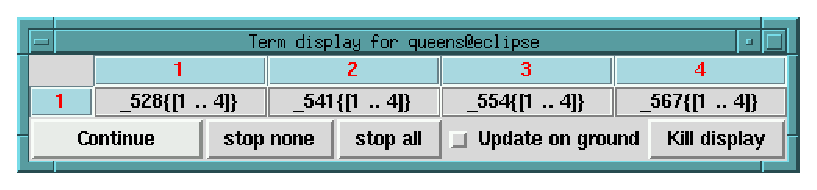
\includegraphics{dismat.eps}
\end{center}
\caption{Display Matrix Tool for 4-Queens (Initial)}
\label{dismat}
\end{figure}

\begin{figure}[bt]
\begin{center}
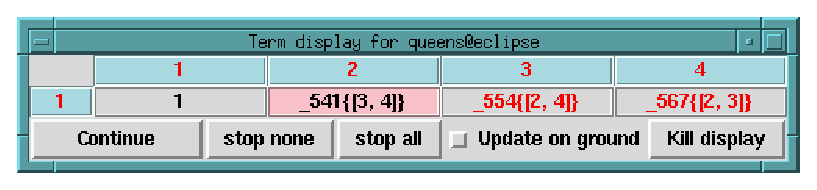
\includegraphics{dismat2.eps}
\end{center}
\caption{Display Matrix Tool for 4-Queens (During execution)}
\label{dismat2}
\end{figure}

Figures~\ref{dismat} and \ref{dismat2} show the tool
invoked with the example N-Queens programs for 4 Queens, at the start
initially and during the execution of the program. The name of the display
window is specified by the second argument of
\bipref{make_display_matrix/2}%
{../bips/kernel/debug/make_display_matrix-2.html},
along with the module it is in. The values of the terms are shown in the
matrix, which can be one dimensional (as in this case), or two
dimensional. Spy points can be set on each individual cell of the matrix
so that execution will stop when the cell is updated. The matrix can be
killed using the `Kill display' button. Left-clicking on a cell will bring
up a menu which shows the current and previous value of the term in the
cell (the current value is shown because the space available in the cell
may be too small to fully display the term), and allows the user to inspect
the term using the inspector.

Note that the display matrix can be used independently of, or in conjunction
with, the tracer. Multiple display matrices can be created to view
different terms.

The following predicates are available in conjunction with the display
matrix:

\medskip
\begin{quote}
\preddef{make_display_matrix(+\pattern{Terms},~+\pattern{Name})}%
\indextt{make_display_matrix/2}\\
\preddef{make_display_matrix(%
+\pattern{Terms},~+\pattern{Prio},~+\pattern{Type},%
~+\pattern{CondList},~+\pattern{Name})}%
\indextt{make_display_matrix/5}
\end{quote}

These
predicates create a display matrix of terms that can be monitored under
{\tkeclipse}. The two argument form is a simplification of the five argument
form, with defaults settings for the extra arguments.
\about{Terms} is a list or
array of terms to be displayed.
A list \about{List} can be specified in the form \pattern{List/N},
where \about{N} is the number of elements per row of the matrix.
If \about{N} is 0, then
the list will be displayed in one row (it could also be omitted in this
case). The extra arguments are used to control how the display is updated.

   The terms are monitored by placing a demon suspension on the variables
   in each term. When a demon wakes, the new value of the term it is
   associated with is sent to the display matrix (and possibly updated,
   depending on the interactive settings on the matrix). When the new
   value is retracted during backtracking,
   the old value is sent to the display matrix.
   The other arguments in this predicate are used to control when the
   demon wakes, and what sort of information is monitored. \about{Prio} is the
   priority that the demon should be suspended at, \about{Type} is designed to
   specify the attributes that are being monitored (currently all
   attributes are monitored, and
   \about{Type} is a dummy argument), \about{CondList} is
   the suspension list that the demon should be added to. Depending on
   these arguments, the level of monitoring can be controlled. Note that
   it is possible for the display matrix to show values that are out of
   date because the change was not monitored.

   The display matrix will be removed on backtracking. However, it will
   not be removed if \predspec{make_display_matrix} has been
   cut: \predspec{kill_display_matrix/1} can be used to explicitly remove
   the
   matrix in this case.

\medskip
\begin{quote}
\preddef{kill_display_matrix(+\pattern{Name})}%
\indextt{kill_display_matrix/1}
\end{quote}

This predicate destroys an existing
   display matrix. \about{Name} is an atomic term which identifies the matrix.

   Destroys an existing display matrix. The display matrix is removed
   from being displayed.


\subsection{Invoking display matrix tool interactively}

Display matrices can be created interactively when a program is
executing, if the program is being debugged with the tracer tool. The user
can select terms that are to be observed by a display matrix while at a
debug port. This can be done from the inspector, the tracer, and the delay
goal tools. See the online help files (available from the help menu of
{\tkeclipse}) for more details.

\section{Using the development tools in applications}

The user can develop their own {\eclipse} applications using the
development tools independently of the {\tkeclipse} toplevel. There are two
ways to do this, depending on if the user is also using the embedding Tcl/Tk
interface (see the Embedding and Interfacing Manual) to provide a graphical
front end:

\begin{itemize}
\item The user is using the embedding Tcl/Tk interface, and is thus
developing a graphical front end in Tk. In this case the user can use the
 development tools via the embedding interface. This is described in
 section~\ref{embedtools}.
\item The user is not using the embedding Tcl/Tk interface. In this case
 the user can use the development tools remotely, by using the remote_tools
 library. This is described in section~\ref{useremotetools}.
\end{itemize}

\subsection{Using the Development tools in the Tcl/Tk Embedding Interface}
\label{embedtools}

 The development tool suite was
designed to be independent of the {\tkeclipse} top-level so that they can be
used in a user's application. In effect, the user can replace the
{\tkeclipse}
top-level with their own alternative top-level. Two simple examples in
which this is done are provided in the \verb'lib_tcl' library as
\verb'example.tcl' and \verb'example1.tcl'. In addition, \verb'tkeclipse'
itself, in the file \verb'tkeclipse.pl', can be seen as a more complex
example usage of the interface.

In order to use the Tcl/Tk interface, the system must be initialized as
described in the Embedding manual. In addition, the user's Tcl code should
probably also be provided as a package using Tcl's package facility, in
order to allow the program to run in a different directory. See the
Embedding manual and the example programs for more details on the
initialization needed.

The user should most likely provide a connection for the output stream
of {\eclipse} so that output from {\eclipse} will go somewhere in the GUI. In
addition, especially during the development, it is also useful to connect
the error stream to some window so that errors (such as {\eclipse}
compilation errors) are seen by the user. This can be done using the
\verb'ec_queue_connect' Tcl command described in the embedding manual.

Output from {\eclipse} need not be sent to a Tk window directly. The Tcl/Tk
code which receives the output can operate on it before displaying it. It
is intended that all such graphical operations should be performed on the
Tcl side, rather than having some primitives provided on the {\eclipse} side.


The user can also provide balloon-help to his/her own application. The
balloon help package is part of the Megawidget developed by Jeffrey Hobbs
and used in {\tkeclipse}. In order to define a balloon help for a particular
widget, the following Tcl code is needed:

\begin{quote}
\begin{verbatim}
balloonhelp <path> <text>
\end{verbatim}
\end{quote}

\noindent
where \verb'<path>' is the pathname of the widget, and \verb'<text>' is the
text that the user wants to display in the balloon.


\subsection{Using the Remote Development Tools}
\label{useremotetools}

The user can also use the development tools via the remote_tools
library. In this case, the development tools are run as a separate program
from the {\eclipse} session, and are attached to it via the Tcl/Tk remote
interface (see the Embedding and Interfacing Manual). This allows any
{\eclipse} session to use the development tools,
as long as there is the capability for graphical display.

The main purpose for the remote_tools library is to allow the user to
use the development tools in situations where (s)he cannot use the Tcl/Tk
embedding interface, e.g., if {\eclipse} is already embedded into another
programming language, or if the user has to use the tty interface for
{\eclipse}.

\begin{figure}[bt]
\begin{center}
\centering{
\mbox{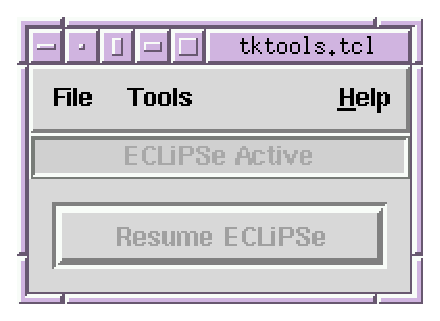
\includegraphics{remotetools.eps}}
\mbox{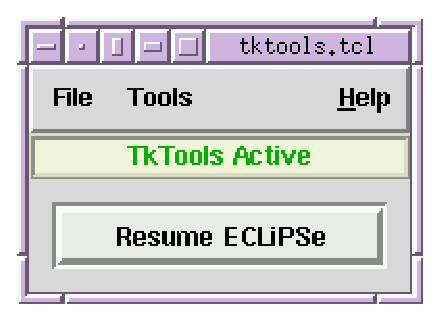
\includegraphics{remotetools2.eps}}
}
\end{center}
\caption{Remote Development Tools Toplevel (left: {\eclipse} active; right:
remote tools active)}
\label{remotetools}
\end{figure}

Once attached to an {\eclipse} session, the remote development tools have
their own window as shown in Figure~\ref{remotetools}. The Tools menu is the
same as in {\tkeclipse}, providing access to the same suite of development
tools. The main body of the window consists of one button and a status
indicator. The indicator shows whether the tools can be used or not (the
tools cannot be used when the {\eclipse} is active), and the button
is used to pass control explicitly to {\eclipse}.

The {\eclipse} session and the development tools are two separate processes
(and in fact they can be running on different machines) that are connected
to each other via the remote Tcl/Tk interface. The interactions of the two
processes are synchronised in that there is a thread-like flow of control
between them: only one process can be `active' at any time. The interaction
is similar to the standard interaction between a debugger and the program
being debugged -- debugging commands can only be issued
while the execution of the program is suspended. In the same way, the user
can only interact with the remote tools window when execution in the
{\eclipse} session is suspended. The toplevel window of the remote tools
has an indicator showing which side has control (see Figure~\ref{remotetools}).
To allow {\eclipse} to resume execution, control is transferred back from
the remote tools to {\eclipse}. This can either be
done automatically from the tools (e.g., when one of the debug buttons is
pressed in the tracer tool), or control can be transferred explicitly back
to {\eclipse} via the ``Resume ECLiPSe'' button on the remote tools window.


\subsubsection{Starting Remote Tools}

To use the remote tools, the user must first load the right library
with \verb'lib(remote_tools)'. After loading the library, the user can
start the remote tools by
starting the development tools as a separate program and then manually
attaching the program to the {\eclipse} session. This allows the development
tools to be run on a different machine from the {\eclipse} session. In this
case, the user initiates the attachment in {\eclipse} with
\bipref{attach_tools/0}{../bips/lib/remote_tools/attach_tools-0.html}:

\begin{quote}
\begin{verbatim}
[eclipse 2]: attach_tools.
Socket created at address holborn.icparc.ic.ac.uk/22849
\end{verbatim}
\end{quote}

{\eclipse} prints the host and port address it expects the remote tools to
attach to, and execution is now suspended waiting for the remote tools to
attach. This is done by running the \toolname{tktools} program, which is located
with the other {\eclipse} executables. As stated, this program can be run
on a different machine from the {\eclipse} session, as long as the two are
connected via a network such as the internet. A connection window is then
displayed as shown:
\vfill %<<<<<<<<<<<

\begin{center}
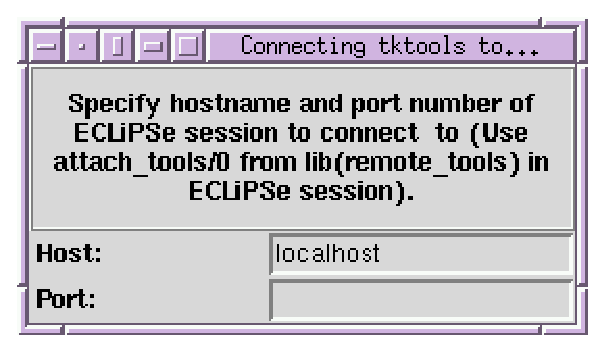
\includegraphics{remotecon.eps}
\end{center}

The same `host' and `port' fields as printed by the {\eclipse} session should
be entered. The default `host' field is `localhost'. This will work if the
remote tools are ran on the same machine as the {\eclipse}
session. Otherwise the full name of the `host' as given by
\predspec{attach_tools/0} must be entered:

\begin{center}
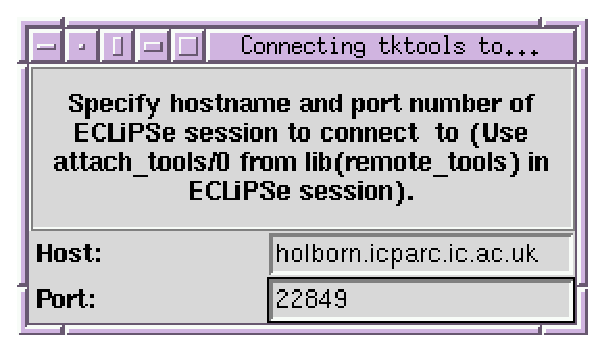
\includegraphics{remotecon2.eps}
\end{center}

Typing return in the `port' field will start the attachment, and with
success, the remote tools window (see Figure~\ref{remotetools}) will be
displayed. The \predspec{attach_tools/0} predicate will also return.

The user is not able to immediately interact directly with the remote
tools, as the {\eclipse} session is initially given control. The user can
use the {\eclipse} session normally, with the additional availability of
the development tools. For example, the display matrix predicates can be
used as in {\tkeclipse}. Also, the tracer tool replaces the previous
tracing facilities of the {\eclipse} session (this would typically be the
command-line debugger).

The tools can be triggered by events in the {\eclipse} session as described
above. In order to use the tools in a more interactive way, control should
be handed over to the remote tools. This can be done by calling the
\bipref{tools/0}{../bips/lib/remote_tools/tools-0.html} predicate.
When the remote tools have control, the user can
now interactively select development tools from the Tools menu.

The remote_tools library provides several predicates to facilitate the use
of the remote development tools:

\begin{quote}
\begin{description}
\item[tools\indextt{tools/0}] Explicitly hands over control to the remote
development
tools. The tools window can then be used interactively. Execution on the
{\eclipse} session is suspended until the remote tools allows {\eclipse} to
resume, at which point the predicate succeeds. The predicate will abort if
the development tools are disconnected from the {\eclipse} session.

\item[attached(?\pattern{ControlStream})\indextt{attached/1}]
	Checks if the remote development tools have been attached to this
        {\eclipse} session or not. If attached, the predicate succeeds and
        unifies \about{ControlStream} with the stream name of the control
        stream. If not attached, the  predicate fails.

\end{description}
\end{quote}

Once attached, the remote development tools should be connected until the
user quits the session. Although it is possible to disconnect the tools
from the {\eclipse} session (from the File menu in the development tools
window), this is not recommended, as there would not be any debugging
facilities available after the disconnection -- the original tracer would
not be restored.

It is possible to attach the remote development tools to any {\eclipse}
session, including one that is using the embedding Tcl/Tk interface (and
indeed, to {\tkeclipse} itself). However, using the tools via the embedding
interface is usually the better option if available, because the tools are
more tightly coupled to {\eclipse} in this case. This means that the
communications between {\eclipse} and the tools are more efficient (and
hence something like the display matrix would perform more efficiently).


%HEVEA\cutend

